%%%%%%%%%%%%%%%%%%%%%%%%%%%%%%%%%%%%%%%%%%%%%%%%%%%%%%%%%%%%%%%%%%%%%%%%%%%%%%%%
\chapter{Системотехническая часть}
%%%%%%%%%%%%%%%%%%%%%%%%%%%%%%%%%%%%%%%%%%%%%%%%%%%%%%%%%%%%%%%%%%%%%%%%%%%%%%%%

%%%%%%%%%%%%%%%%%%%%%%%%%%%%%%%%%%%%%%%%%%%%%%%%%%%%%%%%%%%%%%%%%%%%%%%%%%%%%%%%
\section{Анализ предметной области}
\subsection{Интерактивное обучение}
Сам термин «обучение» может трактоваться в педагогике достаточно широко. Одно из наиболее удачных определений звучит так: обучение — это двусторонний процесс, осуществляемый учителем (преподавание) и учащимся (учение) \cite{pedDict}.

В данном контексте необходимо разграничить понятия «обучение» и «познание». Так, первичным относительно процесса обучения является отношение «обучающий — обучаемый», которое порождает отношение «обучаемый — учебный материал», относящееся в свою очередь уже к понятию «познание». То есть, ключевым процессом является процесс познания, а обучение — это часть процесса познания, для которой необходимо наличие учителя.

Схематично модель процесса обучения приведена на рисунке \ref{fig:ed-process}

\begin{figure}[htbp]
\centering
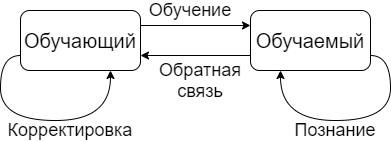
\includegraphics[width=\textwidth]{ed-process.png}
\caption{Модель процесса обучения}%
\label{fig:ed-process}
\end{figure}

Одним из инструментов, использующихся в образовательном процессе, являются автоматизированные обучающие системы (АОС), к которым можно отнести и образовательные платформы. Согласно Полату, АОС — это совокупность связанных в единое целое технических, программно-алгоритмических, лингвистических информационно-методических средств, предназначенных для автоматизации обучающего диалога, поиска и обработки учебной информации \cite{Polat}.

Принято выделять три составляющих АОС:
\begin{itemize*}
\item теоретическую;
\item тренирующую;
\item контролирующую.
\end{itemize*}

Согласно рисунку \ref{fig:ed-process} АОС должны реализовывать некоторую обратную связь. Эта связь может быть двух типов: внутренняя и внешняя.

Внутренняя обратная связь – это информация, которую обучающийся получает от системы в результате своих действий. Она может иметь как консультирующий (помощь, подсказка и т.п.), так и результативный («верно-неверно», демонстрация правильного результата и т.п.) характер.

Внешняя обратная связь – информация, поступающая от обучающей системы к преподавателю. Пользуясь этой информацией, преподаватель может сам корректировать сценарий обучения.

Наличие этой обратной связи и использование подхода, при котором способ подачи материала корректируется в зависимости от полученной информации об успешности освоения этого материала обучающимися позволяет говорить об использовании интерактивных методов обучения.

Среди множества подобных методов принято выделять следующие \cite{Cholak}:
\begin{itemize*}
\item творческие задания;
\item работа в малых группах;
\item работа в парах;
\item обучающие игры (ролевые игры, имитации, деловые игры и образовательные игры)
\item использование общественных ресурсов (приглашение специалиста, экскурсии);
\item социальные проекты и другие внеаудиторные методы обучения (социальные проекты, соревнования, радио и газеты, фильмы, спектакли, выставки, представления, песни и сказки);
\item разминки;
\item изучение и закрепление нового материала (интерактивная лекция, работа с наглядными пособиями, видео- и аудиоматериалами, «ученик в роли учителя», «каждый учит каждого», мозаика (ажурная пила), использование вопросов, Сократический диалог);
\item обсуждение сложных и дискуссионных вопросов и проблем («Займи позицию (шкала мнений)», ПОПС-формула, проективные техники, «Один — вдвоем — все вместе», «Смени позицию», «Карусель», «Дискуссия в стиле телевизионного ток-шоу», дебаты, симпозиум);
\item разрешение проблем («Дерево решений», «Мозговой штурм», «Анализ казусов», «Переговоры и медиация», «Лестницы и змейки»);
\item кейс-метод;
\item презентации.
\end{itemize*}

\subsection{Геймификация в образовании}

В широком смысле геймификация (от англ. gamification, также игрофикация, геймизация) трактуется как использование игровых подходов и механик для расширения неигрового контекста с целью повышения вовлеченности аудитории \cite{gamification}

Сама идея применения подобной стратегии в образовании не нова: про использование игр в обучении писал еще К.Д. Ушинский, на сегодняшний день по этой теме написано множество статей и диссертаций.

Многие исследователи игры отмечают мобилизацию и активизацию возможностей личности, реализацию ее творческого потенциала, так как игре присущи такие характеристики, как импровизация, дух соперничества, эмоциональная составляющая и удовольствие. Являясь развлечением, разрядкой, она способна перерасти в обучение, в творчество, в моделирование человеческих отношений. Значение игровой технологии невозможно исчерпать и оценить развлекательно - рекреативными возможностями. В том и состоит ее феномен, что являясь развлечением, отдыхом, она способна перерасти в обучение, в творчество, в терапию, в модель типа человеческих отношений и проявлений в труде, воспитании. \cite{gamification-ed}

Кроме того, существует ряд исследований \cite{d1, d2} касательно участия дофамина в запоминании информации. Принимая во внимание, что природа процессов, протекающих в мозге человека, изучена далеко не полностью, можно, тем не менее, прийти к следующему упрощению: 

\begin{enumerate}
\item Информация тем надежнее откладывается в долгосрочную память, чем более эмоционально окрашен был момент ознакомления с ней.
\item Положительные эмоции способствуют усвоению информации больше, чем негативные.
\end{enumerate}

\subsection{Визуальное программирование}

Визуальное программирование - способ создания программы для ЭВМ путём манипулирования графическими объектами вместо написания её текста \cite{VPL}.

В ходе изучения материалов для написания данной работы были замечены некоторые расхождения в определении того, что стоит понимать под термином «визуальное программирование». 

Так, например, некоторые источники относят к визуальному программированию средства WYSIWYG проектирования интерфейсов программ, приводя в пример инструменты, подобные тем, которые предлагает среда разработки программного обеспечения Microsoft Visual Studio. Однако, данный набор средств лишь упрощает и делает более предсказуемым разметку элементов графического интерфейса пользователя и предоставляет фрагменты автогенерируемого кода для ведения дальнейшей разработки на языке текстового программирования. Пример такого инструментария приведен на рисунке \ref{fig:wysiwyg}.

\begin{figure}[htbp]
	\centering
	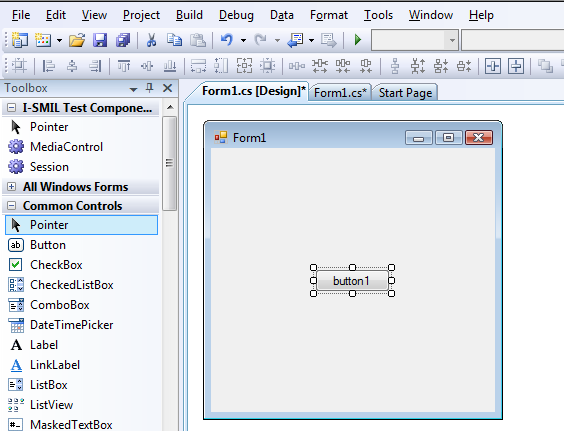
\includegraphics[width=\textwidth]{wysiwyg.png}
	\caption{Визуальный редактор форм для Windows-приложения в среде разработки Microsoft Visual Studio 2008}%
	\label{fig:wysiwyg}
\end{figure}

Также на рынке присутствует значительное количество SCADA и SCADA-подобных систем, наиболее известным представителем которых является программный пакет LabVIEW. В целом данная категория аппаратно-программного обеспечения используется в отрасли АСУ ТП для разработки или обеспечения работы в реальном времени систем сбора, обработки, отображения и архивирования информации об объекте мониторинга или управления. Пример программы, разработанной с помощью LabVIEW приведен на рисунке \ref{fig:labview}.

\begin{figure}[htbp]
	\centering
	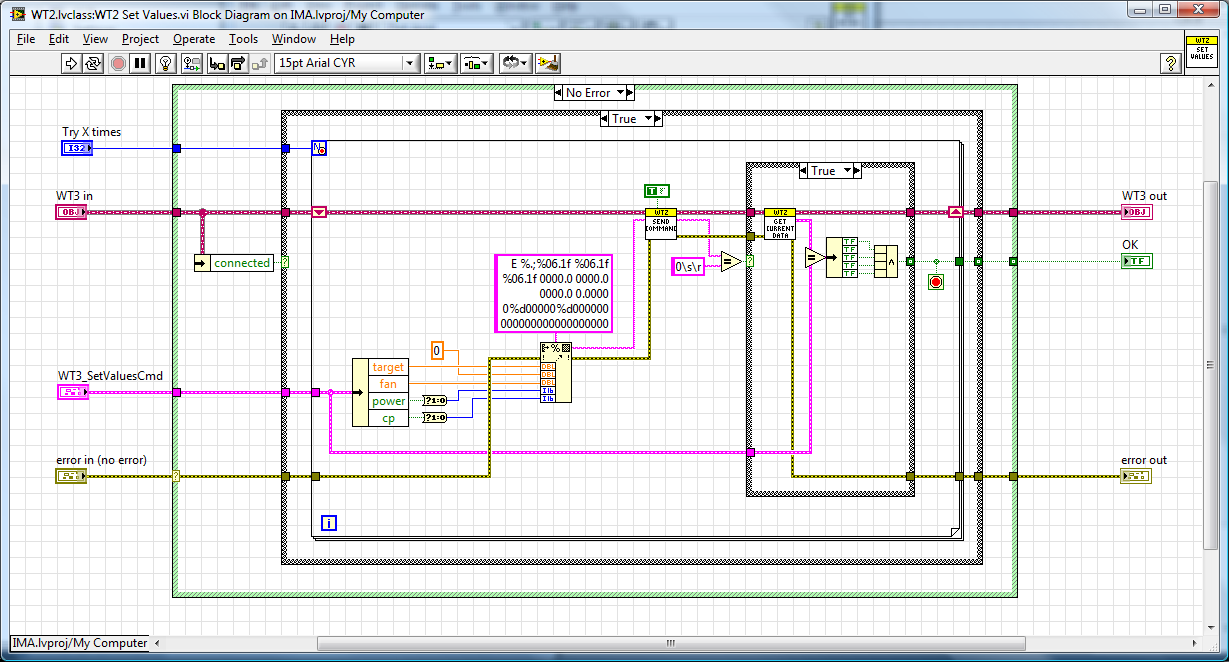
\includegraphics[width=\textwidth]{labview.png}
	\caption{Пример описания программы в среде LabVIEW}%
	\label{fig:labview}
\end{figure}

В частности, используемый в LabVIEW язык визуального программирования G основан на парадигме программирования потоков данных. Графическим представлением данного подхода может служить диаграмма потоков данных (Dataflow Diagram, DFD), приведенная на рисунке \ref{fig:dfd}.

\begin{figure}[htbp]
	\centering
	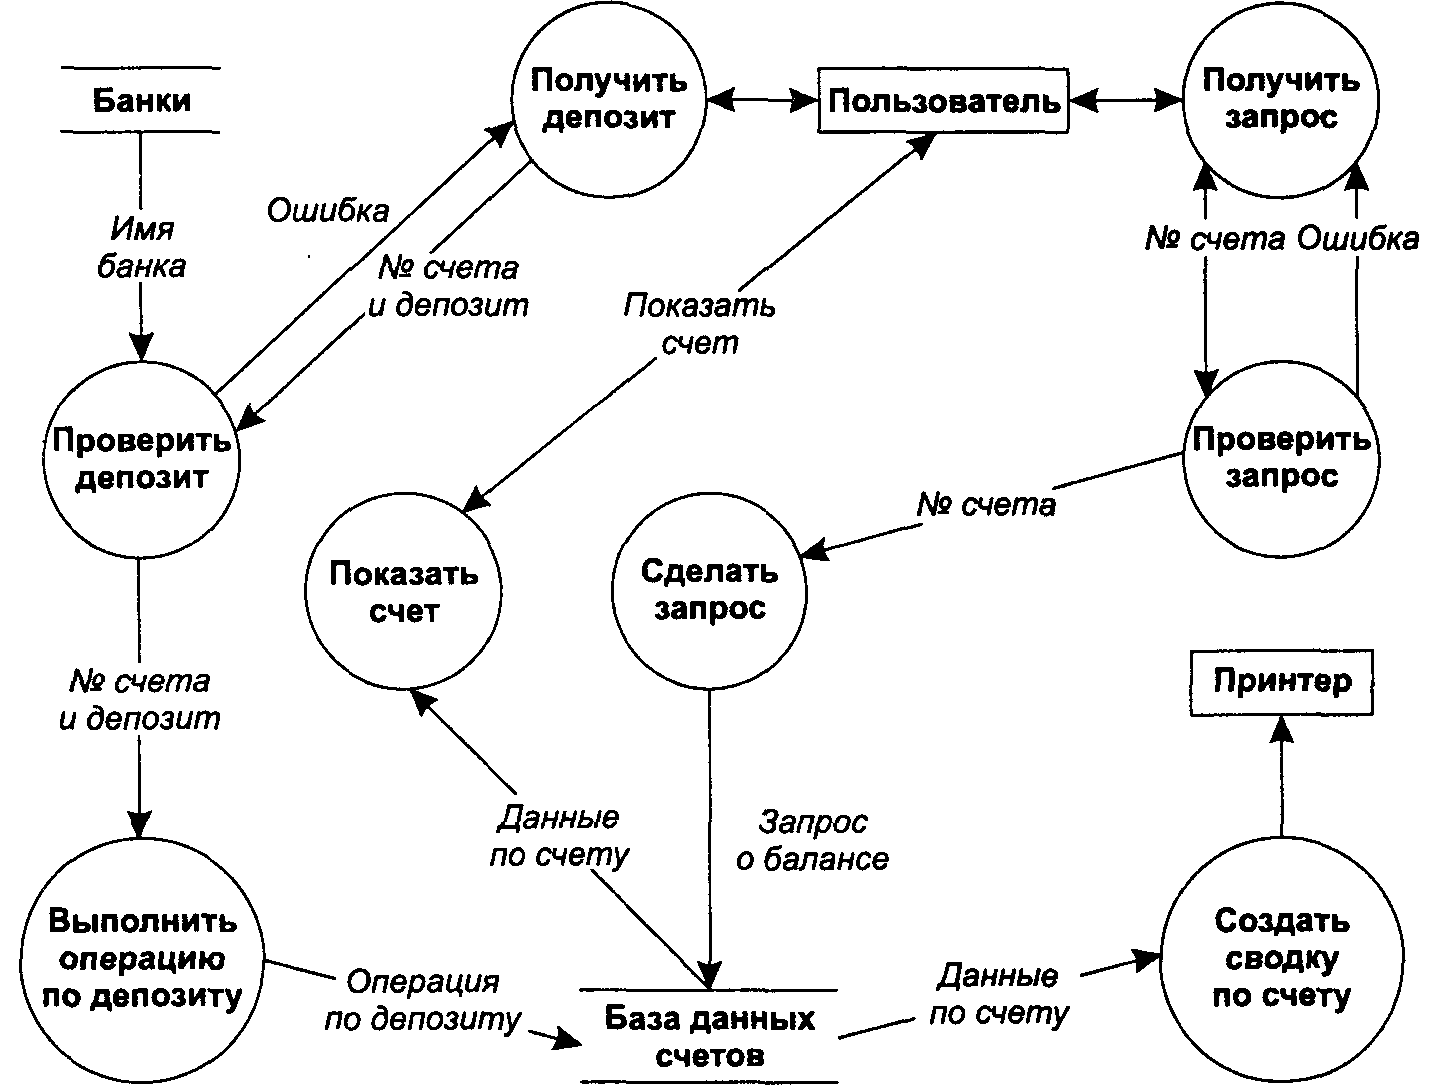
\includegraphics[width=\textwidth]{dfd.png}
	\caption{Диаграмма потоков данных}%
	\label{fig:dfd}
\end{figure}

Подобно DFD, нотация UML (Unified Modeling Language, унифицированный язык моделирования) также активно используется для моделирования бизнес-процессов и системного проектирования. Пример UML диаграммы вариантов использования продемонстрирован на рисунке \ref{fig:uml}. Существуют решения \cite{uml} для генерации кода из UML в языки текстового программирования, однако, данная практика, подобно рассмотренным выше WYSIWYG-редакторам не может расцениваться как программирование в чистом виде, являясь, тем не менее, зарекомендовавшим себя инструментом моделирования и документирования разрабатываемых систем.

\begin{figure}[htbp]
	\centering
	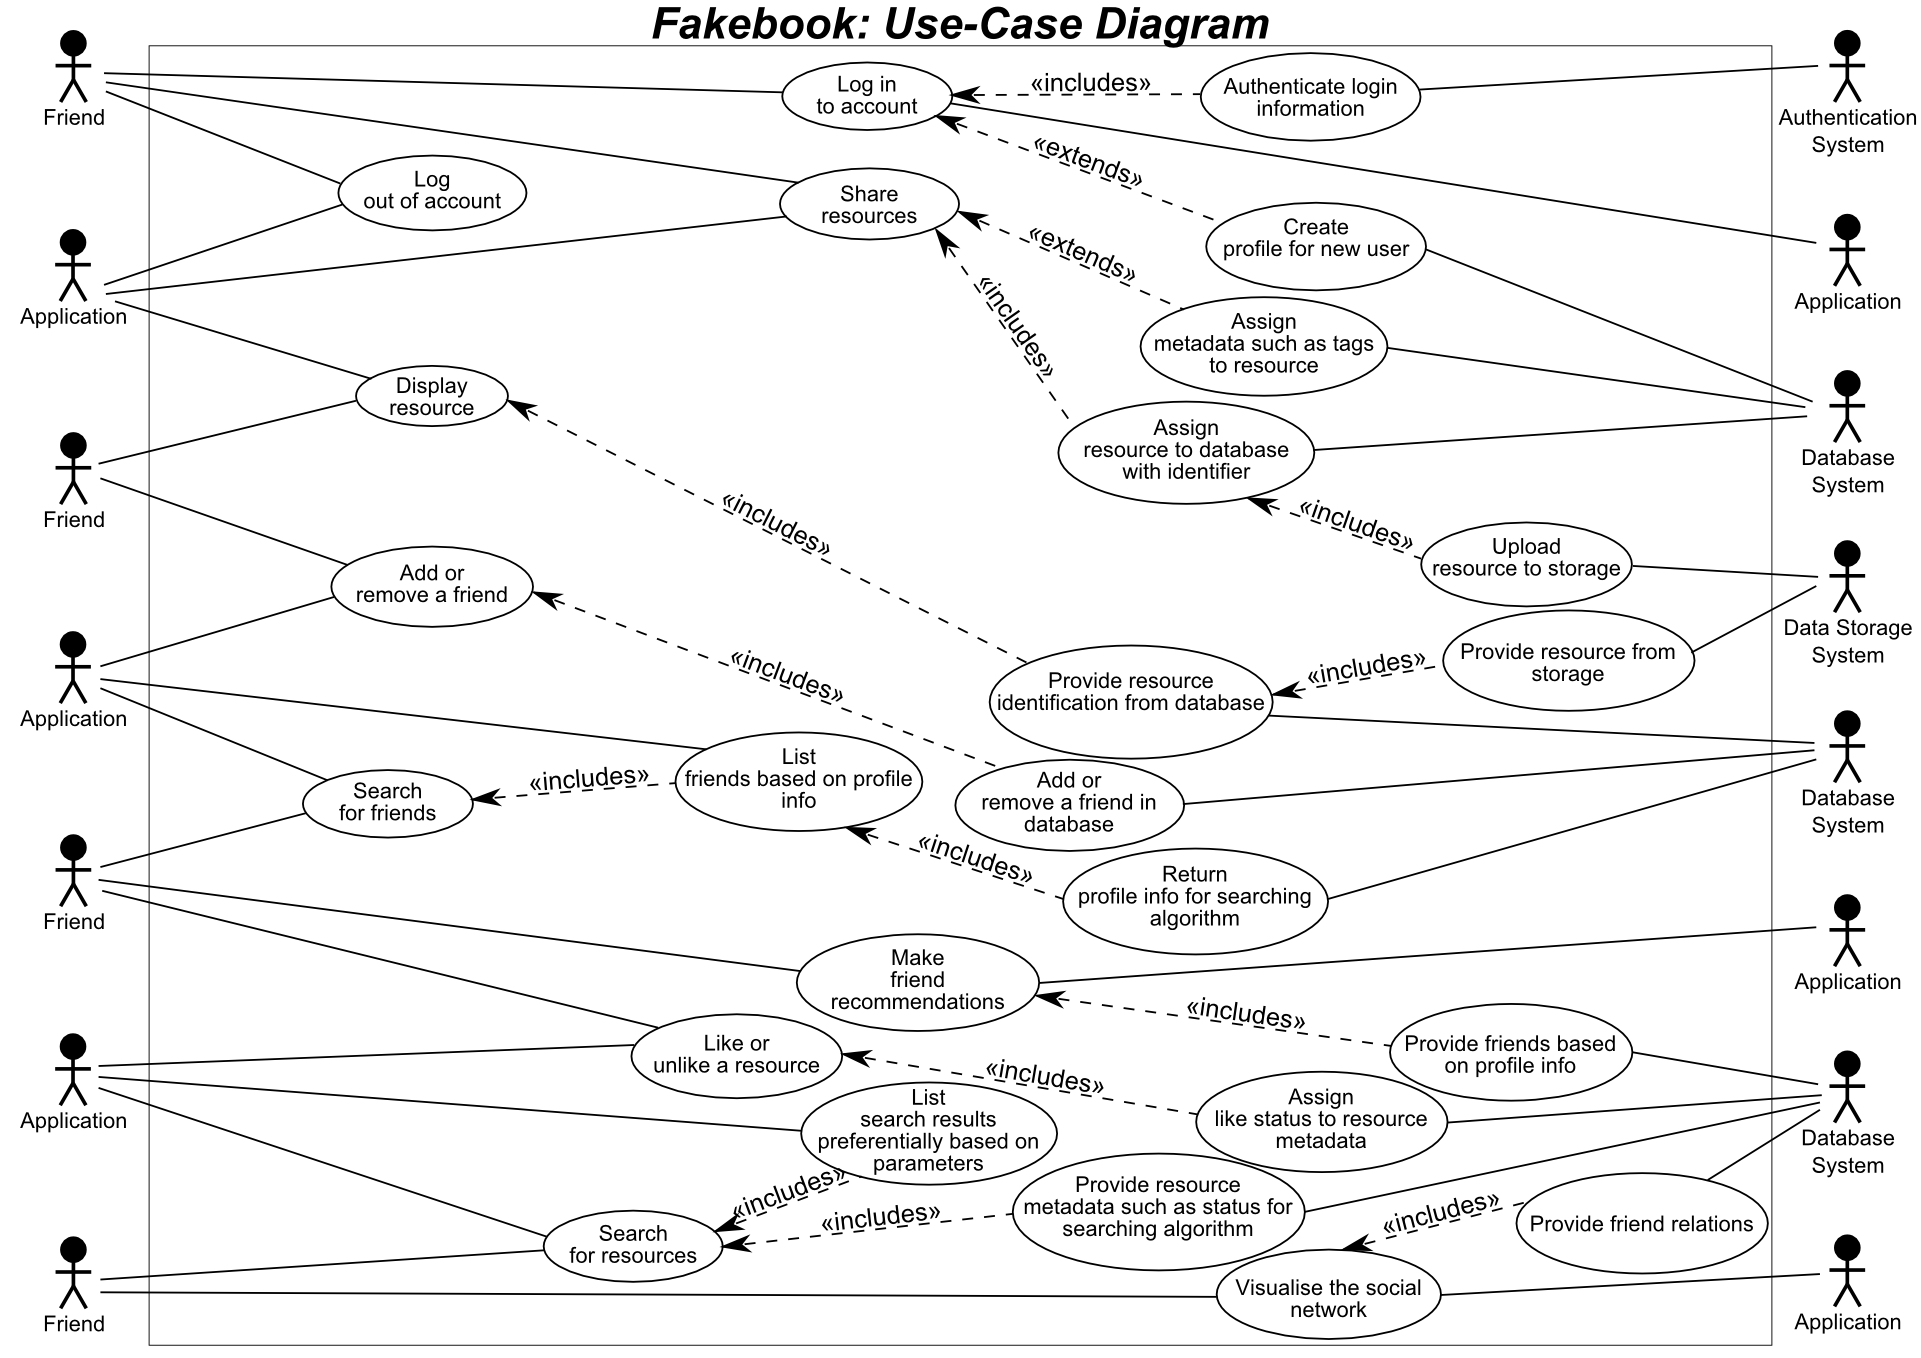
\includegraphics[width=\textwidth]{uml.png}
	\caption{Диаграмма вариантов использования}%
	\label{fig:uml}
\end{figure}

Еще одним примером использования визуального программирования является Blueprint, используемый для взаимодействия с игровым движком Unreal Engine. Пример сценария с использованием этой технологии приведен на рисунке \ref{fig:bp}. Blueprint, в первую очередь, по причине низкой производительности \cite{bptb} не был введен с целью заменить C++, являющийся основным языком программирования, используемым в движке. Его цель - упростить проектирование высокоуровневых взаимодействий с использованием API Unreal Engine. Сравнение производительности Blueprint и C++ приведено в таблице \ref{table:bptb}.

\begin{figure}[htbp]
	\centering
	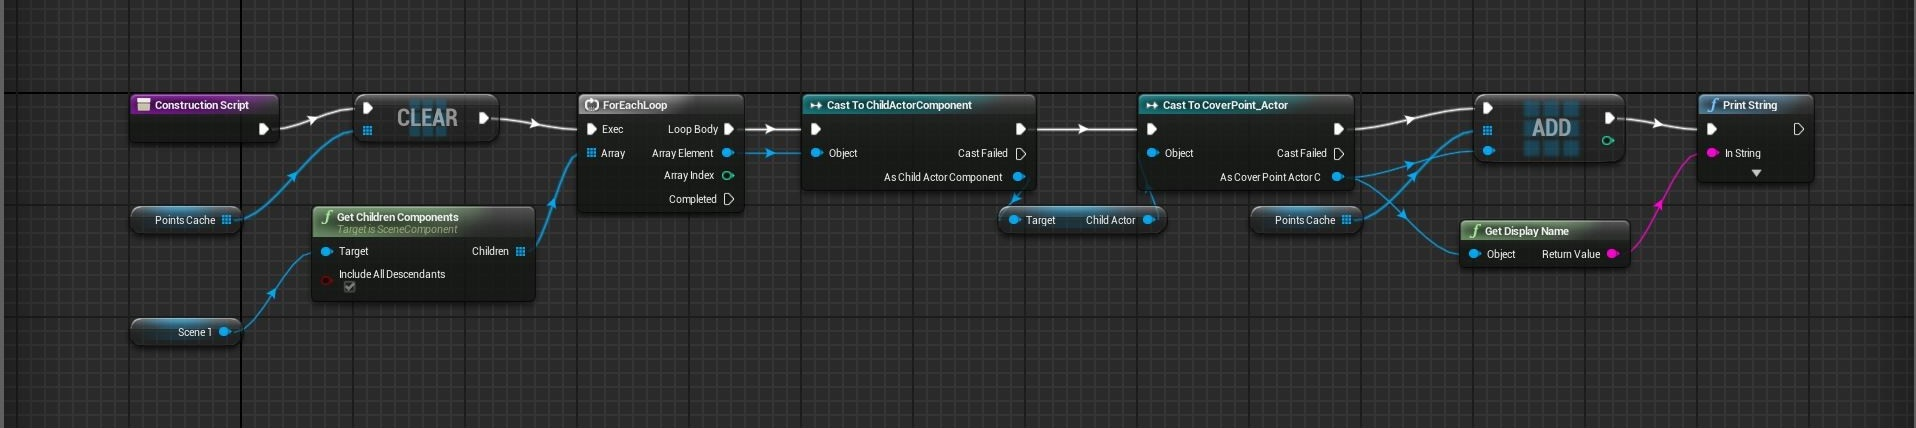
\includegraphics[width=\textwidth]{bp.jpg}
	\caption{Пример сценария, описанного на языке Blueprint}%
	\label{fig:bp}
\end{figure}

\begin{table}
% Для таблиц с multirow и multicol необходимо вручную указать сдвиг для caption
\captionsetup{skip=5pt}
\caption{Сравнение производительности Blueprint и C++}
\centering
\begin{tabular}{|r|c|c|c|c|}
\hline
            \multirow{2}{*}{} 
           & \multicolumn{4}{c|}{Количество итераций} \\ \cline{2-5}
Время обработки, мс & 500   & 1000  & 10000 & 100000  \\ \hline
C++		  			& 0    	& 1     & 50    & 4971     \\ \hline
Blueprint \& C++	& 3    	& 5     & 94    & 5437     \\ \hline
Blueprint			& 454   & -     & -     & -      \\ \hline
\end{tabular}
\label{table:bptb}
\end{table}

Наконец, визуальное программирование активно используется в образовательных целях, поскольку позволяет обучающемуся сконцентрироваться непосредственно на проектировании алгоритмов, скрывая от него аспекты, связанные с конкретной платформой и тонкостями реализации транслятора или виртуальной машины. Конкретные примеры из этой категории будут рассмотрены ниже.

Критика визуального программирования применительно к промышленной разработке программного обеспечения сводится, в основном, к следующим моментам \cite{vpl-crit}:

\begin{itemize*}
	\item недостаточный набор средств поддержки программирования (IntelliSense, статические анализаторы и т.п.);
	\item затрудненный контроль версий в силу большого количества параметров, не относящихся непосредственно к функциональности программ (например, положения блоков);
	\item неоправданно большой визуальный объем программы, поскольку в большинстве случаев одна строка кода на текстовом языке программирования эквивалента нескольким блокам в виузальном языке.
\end{itemize*}

Таким образом, можно выделить следующие области применения визуального программирования:

\begin{enumerate*}
	\item SCADA-подобные системы;
	\item обучение программированию;
	\item моделирование процессов.
\end{enumerate*}

\section{Обзор аналогов}
\subsection{Blockly}
Blockly - это библиотека для создания редакторов визуального программирования от компании Google, написанная на javascript \cite{blockly}.

Технология используется в таких проектах, как App Inventor \cite{app-inventor}, Varwin \cite{varwin}, AutoBlocks for Jira \cite{autoblocks} и многих других. Визуально Blockly крайне схож с решением от лаборатории антидисциплинарных исследований Массачусетского технологического института Scratch \cite{scratch}, однако официальной информации об их связи найти не удалось, хотя веб-сайт упомянутого на официальной странице Google Developers \cite{blockly} в числе продуктов, использующих Blockly, App Inventor размещен на поддомене того же Массачусетского технологического института.

Интерфейс приложения, использующего библиотеку Blockly, продемонстрирован на рисунке \ref{fig:blockly}.

\begin{figure}[htbp]
	\centering
	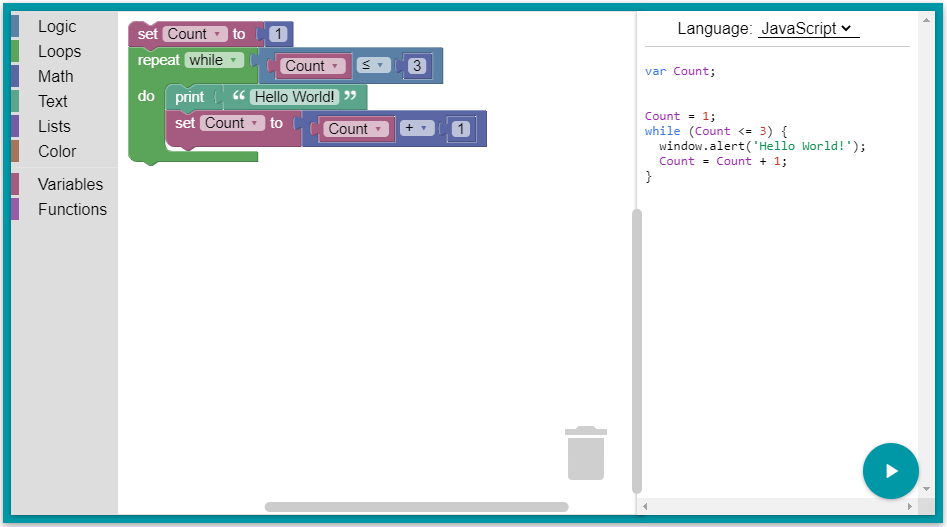
\includegraphics[width=\textwidth]{blockly.png}
	\caption{Интерфейс приложения, использующего библиотеку Blockly}%
	\label{fig:blockly}
\end{figure}

Blockly написан на чистом javascript, не имеет побочных зависимостей и работает полностью на стороне клиента. Составленная программа может компилироваться в такие текстовые языки, как JavaScript, Python, PHP, Lua и Dart.

Блоки, из которых составляется программа, разделены по категориям:

\begin{itemize*}
	\item логические
	\begin{itemize*}
		\item ветвление (if, else, else if);
		\item сравнение (больше, меньше, равно и т.п.);
		\item логическая операция;
		\item отрицание;
		\item логическая константа;
		\item пустое значение (\lstinline|null|);
		\item тернарный оператор (\lstinline|?:|);	
	\end{itemize*}
	\item циклы
	\begin{itemize*}
		\item for;
		\item while;
		\item for .. in;
		\item break/continue;
	\end{itemize*}
	\item математика
	\begin{itemize*}
		\item числовой литерал;
		\item бинарная арифметическая операция;
		\item унарная арифметическая операция;
		\item тригонометрическая функция;
		\item константа ($\pi$, $\sqrt{2}$ и пр.);
		\item проверка числа на принадлежность подмножеству (четные, нечетные, простые и т.п.);
		\item округление;
		\item математические операции над массивами чисел;
		\item остаток от деления;
		\item случайное число;
	\end{itemize*}
	\item списки
	\begin{itemize*}
		\item объявление коллекции;
		\item длина коллекции;
		\item поиск элемента;
		\item CRUD-операции с элементами;
		\item преобразования к строкам;
		\item сортировка;
	\end{itemize*}
	\item цвет
	\begin{itemize*}
		\item константа;
		\item случайный цвет;
		\item смешение цветов;
		\item цвет из RGB-составляющих;
	\end{itemize*}
	\item переменные
	\begin{itemize*}
		\item объявление;
		\item присваивание;
		\item ссылка на переменную;
	\end{itemize*}
	\item функции.
\end{itemize*}

Недостатки Blockly, в целом, сводятся к общей критике визуальных языков программирования, которая была рассмотрена выше. Кроме того, изначально одинаковые конструкции, например, стандартный цикл for, имеют реализацию в виде различных блоков, что может вызывать неточные ассоциации относительно языков, имеющих широкое распространение в коммерческой разработке, что, однако не является недостатком при выбранном подходе, целью которого видится максимальное абстрагирование от конкретного синтаксиса с целью концентрации на алгоритмах в целом.

\subsection{TRIK Studio}

ТРИК - это кибернетический конструктор отечественной разработки. В комплект входят учебные материалы, контроллер, металлический конструктор, а также программное обеспечение \cite{trik}. Важной частью этого программного обеспечения является среда разработки TRIK Studio. 

Среда предназначена для написания программы для собранного из конструктора робота, а также симуляции выполнения этой программы. Интерфейс редактирования программы приведен на рисунке \ref{fig:trik-edit}, симуляции - на рисунке \ref{fig:trik-run}.

\begin{figure}[htbp]
	\centering
	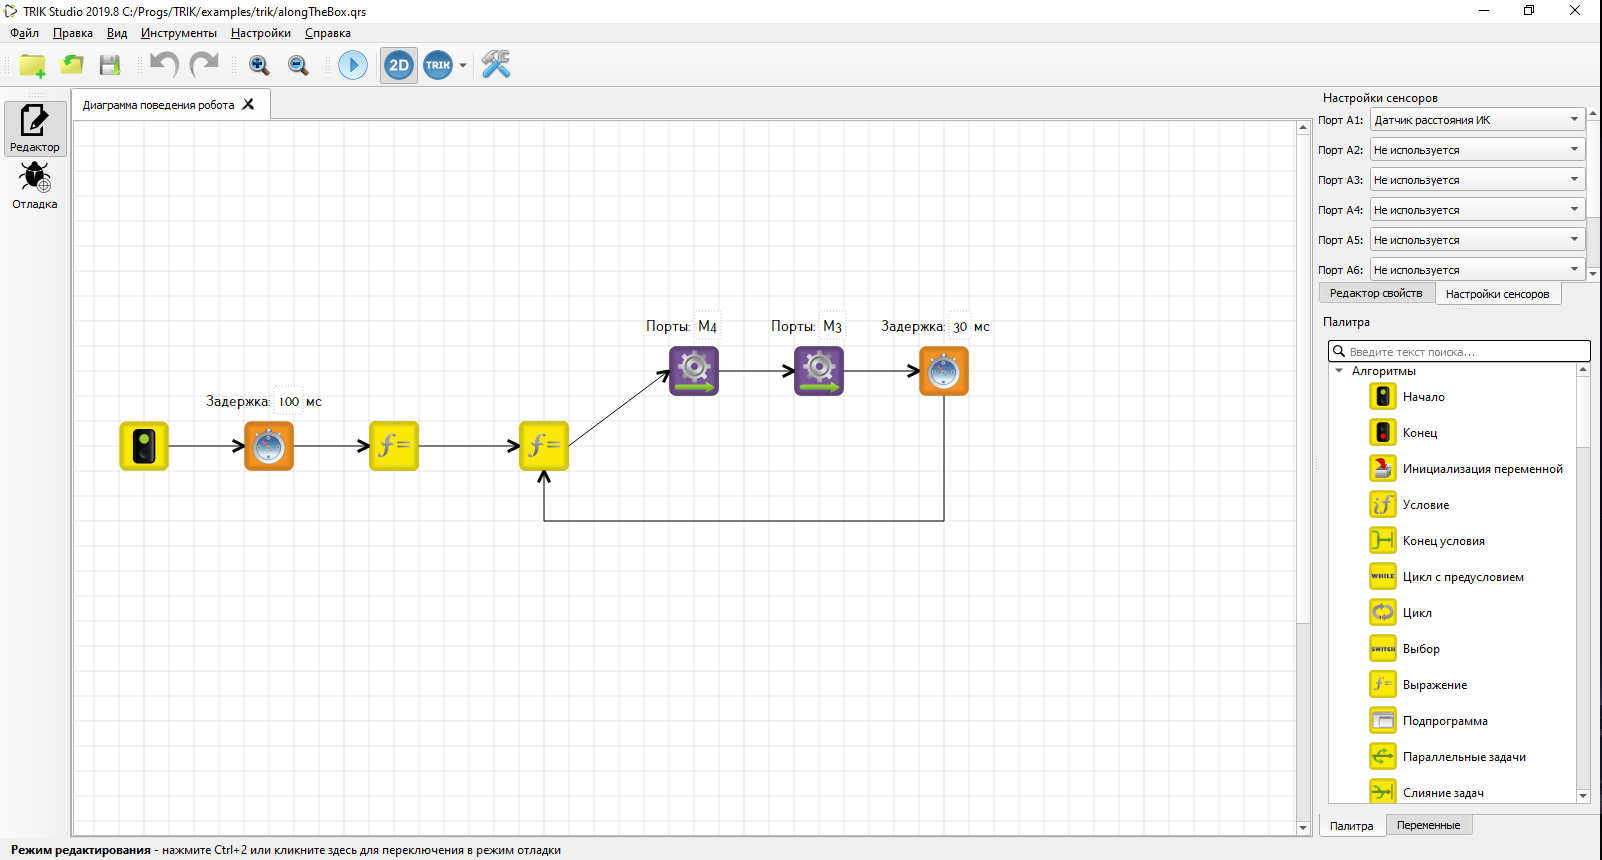
\includegraphics[width=\textwidth]{trik-edit.png}
	\caption{TRIK Studio: режим редактирования}%
	\label{fig:trik-edit}
\end{figure}

\begin{figure}[htbp]
	\centering
	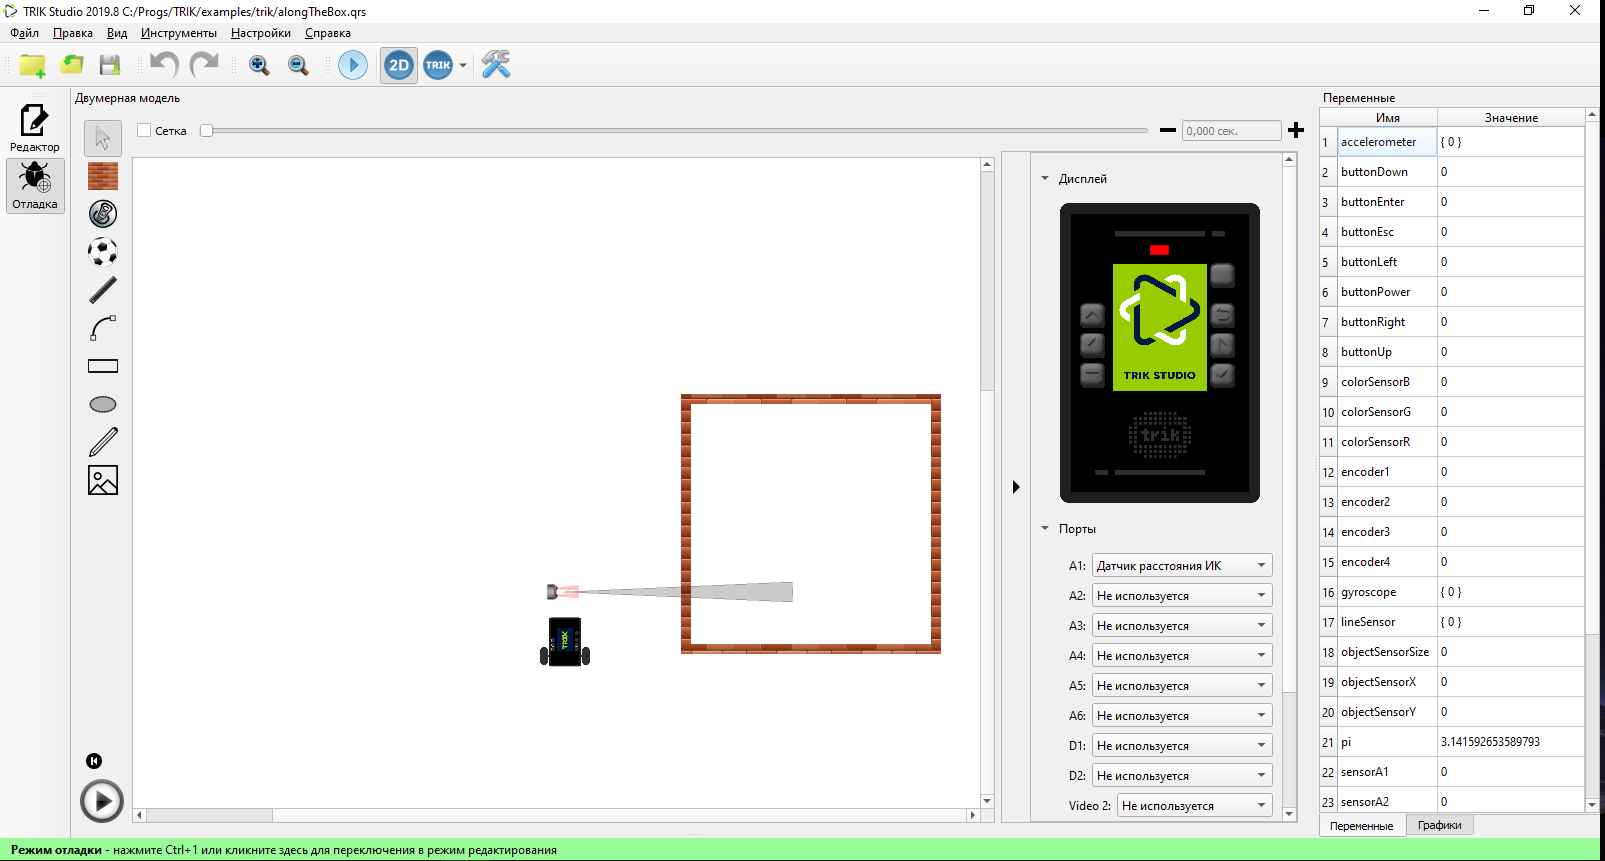
\includegraphics[width=\textwidth]{trik-run.png}
	\caption{TRIK Studio: режим симуляции}%
	\label{fig:trik-run}
\end{figure}

В отличие от компонентов, используемых в библиотеке Blocky, рассмотренной выше, набор блоков, относящихся к алгоритмам, существенно меньше, так как затрагивает алгоритмические абстракции более высокого уровня: начало, конец, цикл, функция, условие и др., зато присутствуют блоки, специфические для аппаратной реализации. Например, поворот робота осуществляется засчет подачи различающихся значений на порты, отвечающие за поведение левого и правого колес робота.

Базовые операции, такие как присваивание, сравнение, арифметические действия осуществляются с помощью текстовых команд, привязанных к соответствующим блокам, что значительно сокращает визуальный объем программы по сравнению с тем же Blockly.

Также при составлении программы разработчик располагает значениями, полученными с датчиков робота, среди которых есть датчики расстояния, освещенности и касания.

Главным достоинством TRIK Studio является относительная универсальность: продукт можно использовать как среду разработки для конкретных аппаратных решений, так и для обучения основам робототехники благодаря встроенной системе симуляции.

Существуют онлайн-курсы \cite{stepik}, которые используют данную среду в качестве программного обеспечения для выполнения домашних заданий. Однако, при таком варианте использования, можно отнести к недостаткам отсутствие бесшовности образовательного процесса, так как для прохождения курса необходимо устанавливать дополнительное программное обеспечение, а также скачивать файлы заданий и загружать результаты выполнения на сервер.

\subsection{Дракон-схемы}

Еще одним примером отечественной разработки в области визуального программирования являются язык ДРАКОН. Пример программы приведен на рисунке \ref{fig:drakon}.

\begin{figure}[htbp]
	\centering
	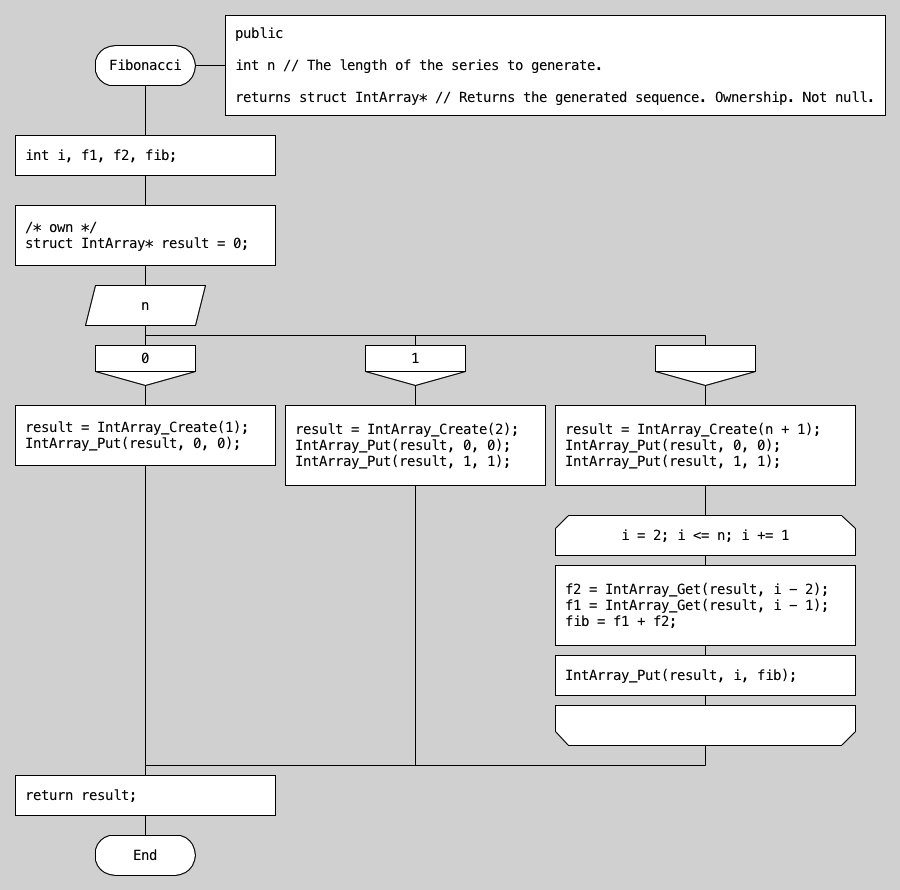
\includegraphics[width=\textwidth]{drakon.png}
	\caption{Вычисление ряда Фибоначчи на языке ДРАКОН}%
	\label{fig:drakon}
\end{figure}

По большому счету, цели, стоявшие перед создателями языка, отражены в его названии: ДРАКОН - дружелюбный русский алгоритмический язык, который обеспечивает наглядность.

Язык разрабатывался с целью замены и объединения функциональности других более узконаправленных языков, используемых при проектировании космического корабля «Буран». Простота понимания была одним из ключевых требований. Так, в книге Владимира Паронджанова приводится следующая цитата: «ДРАКОН — легкий язык. Настолько легкий, что разработку многих компьютерных программ для космических ракет на практике ведут не программисты, а инженеры — по принципу «программирование без программистов». Причина частичного отказа от программистов проста. При решении практических прикладных задач инженеры досконально владеют материалом и прекрасно знают постановку задачи. В отличие от них программисты не знают физику процесса и становятся «лишними людьми», без которых в ряде случаев (хотя и не всегда) вполне можно обойтись.» \cite{drakon}

В языке ДРАКОН присутствуют 27 икон, из которых можно сформировать 21 макроикону. Вместе они формируют алфавит языка ДРАКОН, приведенный на рисунке \ref{fig:drakon-alphabet}.

\begin{figure}[htbp]
	\centering
	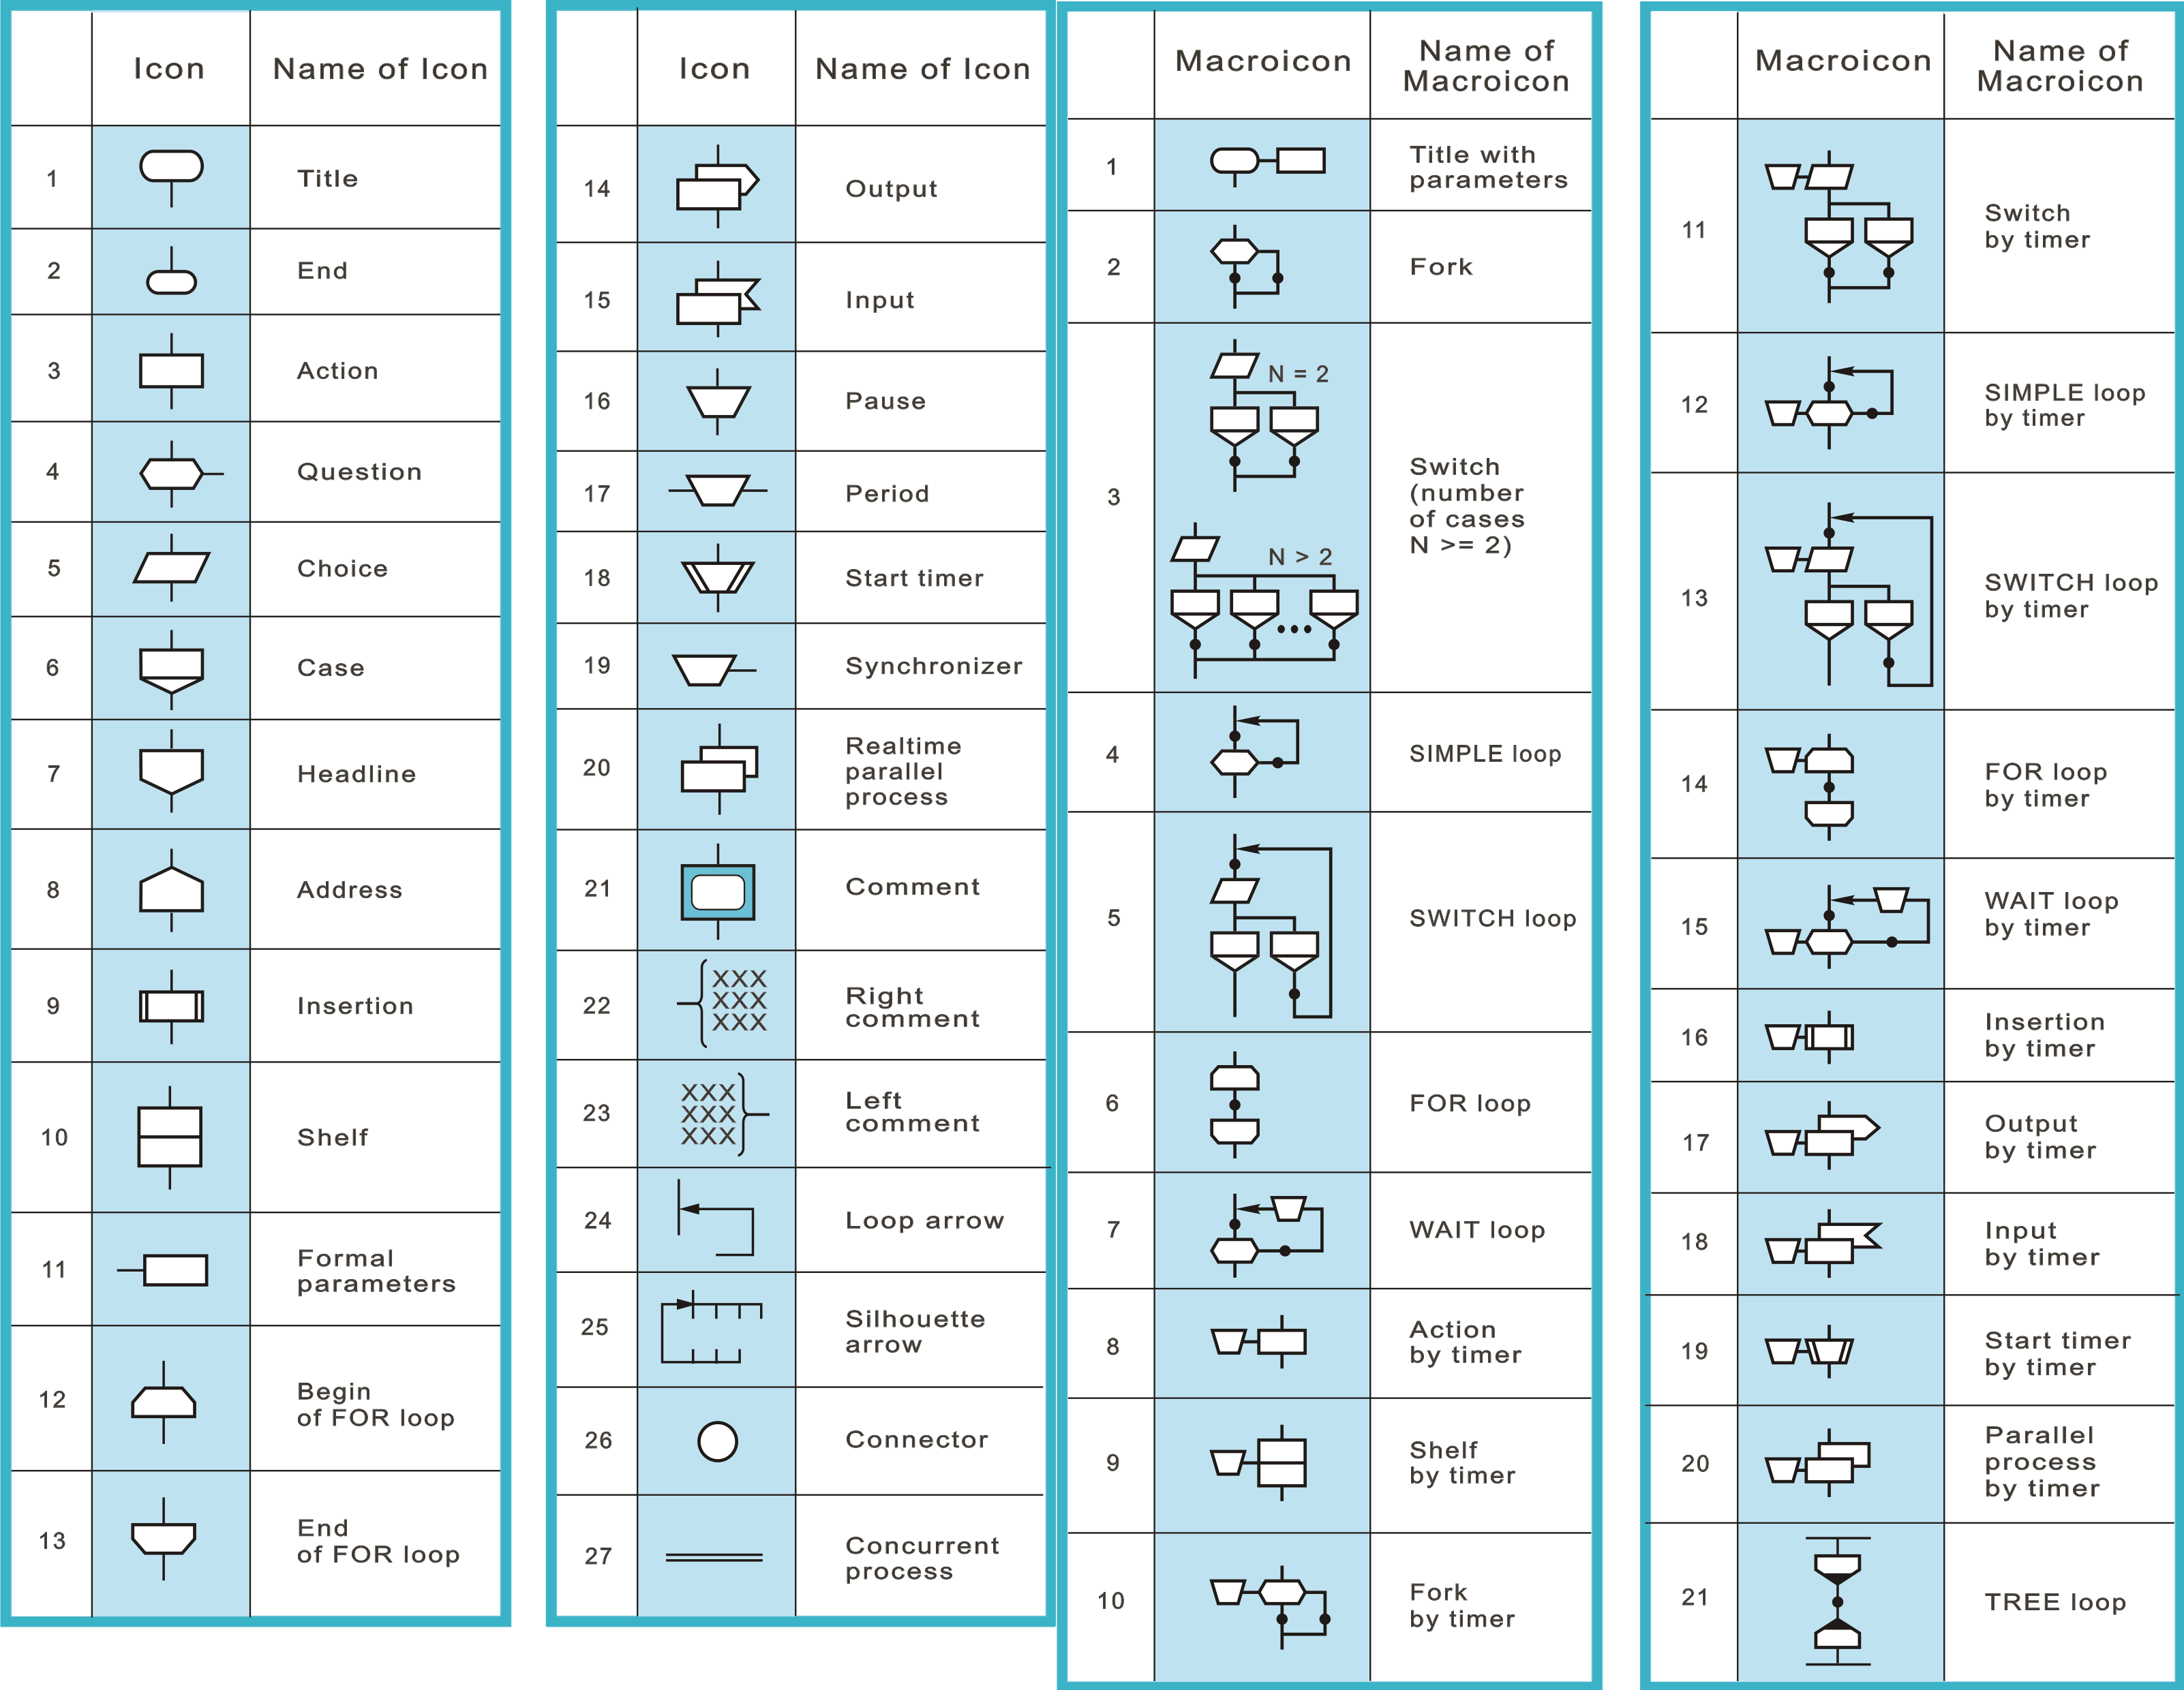
\includegraphics[width=\textwidth]{drakon-alphabet.png}
	\caption{Алфавит языка ДРАКОН}%
	\label{fig:drakon-alphabet}
\end{figure}

В 1975 году в работе «Заметки по структурному программированию» Эдсгер Дейкстра предложил четыре принципа структуризации блок-схем \cite{deixtra}:
\begin{enumerate*}
	\item Принцип ограничения топологии блок-схем. Структурная программа должна приводить «к ограничению топологии блок-схем по сравнению с различными блок-схемами, которые могут быть получены, если разрешить проведение стрелок из любого блока в любой другой блок. Отказавшись от большого разнообразия блок-схем и ограничившись данными тремя типами операторов управления (следование, ветвление, цикл), мы следуем тем самым некоей последовательностной дисциплине».
	\item Принцип вертикальной ориентации входов и выходов блок-схем. Имея в виду шесть типовых блок-схем (if-do, if-then-else, case-of, while-do, repeat-until), Дейкстра пишет: «Общее свойство всех этих блок-схем состоит в том, что у каждой из них один вход вверху и один выход внизу».
	\item Принцип единой вертикали. Вход и выход каждой типовой блок-схемы должны лежать на одной вертикали.
	\item Принцип нанизывания блок-схем на единую вертикаль. Типовые блок-схемы следует соединять между собой, не допуская изломов соединительных линий, чтобы выход верхней и вход нижней блок-схемы лежали на одной вертикали.
\end{enumerate*}

Усовершенствованные согласно рекомендациям Эдсгера Дейкстры блок-схемы языка ДРАКОН называются Дракон-схемами.

Программы, составленные на языке ДРАКОН компилируются в заранее выбранный текстовый язык. Допускается использование текстовых команд выбранного языка внутри блоков. Такое сочетание с целевым текстовым языком называется гибридным языком. Примеры таких сочетаний: ДРАКОН-C, ДРАКОН-Java и другие.

\section{Трансляция текстов программ}
\subsection{Форма Бэкуса-Наура}

Форма Бэкуса-Наура (БНФ) - это формальная система программы синтаксиса, используемая для описания контекстно-свободных грамматик.

Широко используется для описания синтаксиса языков программирования, данных, протоколов и т.д. БНФ подходит как для описания как грамматик, так и регулярного синтаксиса, поскольку регулярные грамматики являются подмножеством контекстно-свободных.

Конструкция БНФ определяет некоторое конечное множество нетерминалов в левой части и правила замены (подстановки) этих нетерминалов другими терминалами или последовательностями символов (терминалами).

Алгоритм проверки на соответствие некоторого текста определенному синтаксису, как правило, выполняется в рекурсивном виде. Кроме того, реализацию такого синтаксиса удобно расширять, поскольку алгоритм легко декомпозируется на отдельные функции, осуществляющие проверки отдельных правил.

Пример описания идентификатора с использованием БНФ приведен в листинге \ref{listings:bnf}

\lstinputlisting[
label={listings:bnf},
caption={Определение идентификатора при помощи БНФ},
]
{listings/bnf.txt}
\subsection{Компиляция}
\subsection{Интерпретация}
\section{API браузера}
\subsection{Очередь задач}
\subsection{Canvas}
%%%%%%%%%%%%%%%%%%%%%%%%%%%%%%%%%%%%%%%%%%%%%%%%%%%%%%%%%%%%%%%%%%%%%%%%%%%%%%%%

%\blindtext
%
%\begin{figure}[htbp]
%\centering
%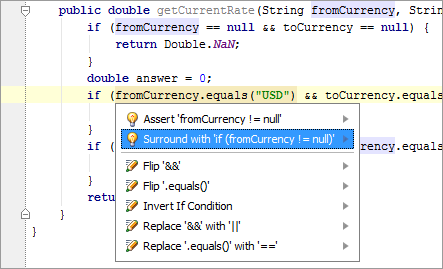
\includegraphics[width=\textwidth]{code_analysis_bugs.png}
%\caption{Рекомендации по проведению исследований в рамках диссертации}%
%\label{fig:how-to-do-research}
%\end{figure}
%
%\Blindtext
%
%\begin{table}
%% Для таблиц с multirow и multicol необходимо вручную указать сдвиг для caption
%\captionsetup{skip=5pt}
%\caption{Example}
%\centering
%\begin{tabular}{|r|c|c|c|c|c|c|}
%\hline
%            \multirow{2}{*}{}
%           & \multicolumn{2}{c|}{LLVM IR} 
%           & \multicolumn{2}{c|}{PS} 
%           & \multicolumn{2}{c|}{AI} \\ \cline{2-7}
%           & SAT    & UNSAT   & SAT    & UNSAT   & SAT    & UNSAT   \\ \hline
%beanstalkd & 356    & 252     & 360    & 161     & 360    & 247     \\ \hline
%clib       & 599    & 258     & 960    & 234     & 960    & 449     \\ \hline
%\end{tabular}
%\label{table:checkResults}
%\end{table}
%
%%%%%%%%%%%%%%%%%%%%%%%%%%%%%%%%%%%%%%%%%%%%%%%%%%%%%%%%%%%%%%%%%%%%%%%%%%%%%%%%%
%\section{bar}
%%%%%%%%%%%%%%%%%%%%%%%%%%%%%%%%%%%%%%%%%%%%%%%%%%%%%%%%%%%%%%%%%%%%%%%%%%%%%%%%%
%
%\blindtext
%It is of great importance that you use correct references in your dissertation.
%Resent studies show that it can increase the chances of successful defense
%by as much as 3,17 percent~\cite{russian, ANTLR, java-book}.
%
%\begin{table}[H]
%	\caption{Название таблицы}
%	\begin{center}
%		\begin{tabular}{|l|l|}
%			\hline
%			top left & top right\\ \hline
%			bot left & bot right\\ \hline
%		\end{tabular}
%		\label{tabular:tab_examp}
%	\end{center}
%\end{table}
%
%
%\Blindtext
